		\documentclass[landscape,final,a0paper,fontscale=0.285]{baposter}
		
		\usepackage{calc}
		\usepackage{graphicx}
		\usepackage{amsmath}
		\usepackage{amssymb}
		\usepackage{relsize}
		\usepackage{multirow}
		\usepackage{rotating}
		\usepackage{bm}
		\usepackage{url}
		\usepackage{color}
		\usepackage{colortbl}

		
		\usepackage{graphicx}
		\usepackage{multicol}
		\usepackage{picture}
		
		%\usepackage{times}
		%\usepackage{helvet}
		%\usepackage{bookman}
		\usepackage{palatino}
		
		\newcommand{\captionfont}{\footnotesize}
		
		\graphicspath{{images/}{../images/}}
		\usetikzlibrary{calc}
		
		\newcommand{\SET}[1]  {\ensuremath{\mathcal{#1}}}
		\newcommand{\MAT}[1]  {\ensuremath{\boldsymbol{#1}}}
		\newcommand{\VEC}[1]  {\ensuremath{\boldsymbol{#1}}}
		\newcommand{\Video}{\SET{V}}
		\newcommand{\video}{\VEC{f}}
		\newcommand{\track}{x}
		\newcommand{\Track}{\SET T}
		\newcommand{\LMs}{\SET L}
		\newcommand{\lm}{l}
		\newcommand{\PosE}{\SET P}
		\newcommand{\posE}{\VEC p}
		\newcommand{\negE}{\VEC n}
		\newcommand{\NegE}{\SET N}
		\newcommand{\Occluded}{\SET O}
		\newcommand{\occluded}{o}

		\newcommand{\eat}[1]{}
		
		%%%%%%%%%%%%%%%%%%%%%%%%%%%%%%%%%%%%%%%%%%%%%%%%%%%%%%%%%%%%%%%%%%%%%%%%%%%%%%%%
		%%%% Some math symbols used in the text
		%%%%%%%%%%%%%%%%%%%%%%%%%%%%%%%%%%%%%%%%%%%%%%%%%%%%%%%%%%%%%%%%%%%%%%%%%%%%%%%%
		
		%%%%%%%%%%%%%%%%%%%%%%%%%%%%%%%%%%%%%%%%%%%%%%%%%%%%%%%%%%%%%%%%%%%%%%%%%%%%%%%%
		% Multicol Settings
		%%%%%%%%%%%%%%%%%%%%%%%%%%%%%%%%%%%%%%%%%%%%%%%%%%%%%%%%%%%%%%%%%%%%%%%%%%%%%%%%
		\setlength{\columnsep}{1em}
		\setlength{\columnseprule}{0mm}
		
		%%%%%%%%%%%%%%%%%%%%%%%%%%%%%%%%%%%%%%%%%%%%%%%%%%%%%%%%%%%%%%%%%%%%%%%%%%%%%%%%
		% Save space in lists. Use this after the opening of the list
		%%%%%%%%%%%%%%%%%%%%%%%%%%%%%%%%%%%%%%%%%%%%%%%%%%%%%%%%%%%%%%%%%%%%%%%%%%%%%%%%
		\newcommand{\compresslist}{%
		\setlength{\itemsep}{1pt}%
		\setlength{\parskip}{0pt}%
		\setlength{\parsep}{0pt}%
		}
		
		%%%%%%%%%%%%%%%%%%%%%%%%%%%%%%%%%%%%%%%%%%%%%%%%%%%%%%%%%%%%%%%%%%%%%%%%%%%%%%
		%%% Begin of Document
		%%%%%%%%%%%%%%%%%%%%%%%%%%%%%%%%%%%%%%%%%%%%%%%%%%%%%%%%%%%%%%%%%%%%%%%%%%%%%%
		
		\begin{document}
		
		%%%%%%%%%%%%%%%%%%%%%%%%%%%%%%%%%%%%%%%%%%%%%%%%%%%%%%%%%%%%%%%%%%%%%%%%%%%%%%
		%%% Here starts the poster
		%%%---------------------------------------------------------------------------
		%%% Format it to your taste with the options
		%%%%%%%%%%%%%%%%%%%%%%%%%%%%%%%%%%%%%%%%%%%%%%%%%%%%%%%%%%%%%%%%%%%%%%%%%%%%%%
		% Define some colors
		
		%\definecolor{lightblue}{cmyk}{0.83,0.24,0,0.12}
		\definecolor{lightblue}{rgb}{0.145,0.6666,1}
		
		% Draw a video
		\newlength{\FSZ}
		\newcommand{\drawvideo}[3]{% [0 0.25 0.5 0.75 1 1.25 1.5]
		   \noindent\pgfmathsetlength{\FSZ}{\linewidth/#2}
		   \begin{tikzpicture}[outer sep=0pt,inner sep=0pt,x=\FSZ,y=\FSZ]
		   \draw[color=lightblue!50!black] (0,0) node[outer sep=0pt,inner sep=0pt,text width=\linewidth,minimum height=0] (video) {\noindent#3};
		   \path [fill=lightblue!50!black,line width=0pt] 
		     (video.north west) rectangle ([yshift=\FSZ] video.north east) 
		    \foreach \x in {1,2,...,#2} {
		      {[rounded corners=0.6] ($(video.north west)+(-0.7,0.8)+(\x,0)$) rectangle +(0.4,-0.6)}
		    }
		;
		   \path [fill=lightblue!50!black,line width=0pt] 
		     ([yshift=-1\FSZ] video.south west) rectangle (video.south east) 
		    \foreach \x in {1,2,...,#2} {
		      {[rounded corners=0.6] ($(video.south west)+(-0.7,-0.2)+(\x,0)$) rectangle +(0.4,-0.6)}
		    }
		;
		   \foreach \x in {1,...,#1} {
		     \draw[color=lightblue!50!black] ([xshift=\x\linewidth/#1] video.north west) -- ([xshift=\x\linewidth/#1] video.south west);
		   }
		   \foreach \x in {0,#1} {
		     \draw[color=lightblue!50!black] ([xshift=\x\linewidth/#1,yshift=1\FSZ] video.north west) -- ([xshift=\x\linewidth/#1,yshift=-1\FSZ] video.south west);
		   }
		   \end{tikzpicture}
		}
		
		\hyphenation{resolution occlusions}
		%%
		\begin{poster}%
		  % Poster Options
		  {
		  % Show grid to help with alignment
		  grid=false,
		  % Column spacing
		  colspacing=1em,
		  % Color style
		  bgColorOne=white,
		  bgColorTwo=white,
		  borderColor=lightblue,
		  headerColorOne=black,
		  headerColorTwo=lightblue,
		  headerFontColor=white,
		  boxColorOne=white,
		  boxColorTwo=lightblue,
		  % Format of textbox
		  textborder=roundedleft,
		  % Format of text header
		  eyecatcher=false,
		  headerborder=closed,
		  headerheight=0.090\textheight,
		  %headerheight=0.125\textheight,
		%  textfont=\sc, An example of changing the text font
		  headershape=roundedright,
		  headershade=shadelr,
		  headerfont=\Large\bf\textsc, %Sans Serif
		  textfont={\setlength{\parindent}{1.5em}},
		  boxshade=plain,
		%  background=shade-tb,
		  background=plain,
		  linewidth=2pt
		  }
		  % Eye Catcher
		  {\includegraphics[height=3em]{images/graph_occluded.pdf}} 
		  % Title
		  {\bf{\underline{Linear-chain CRF for NLP in MADlib}}\vspace{-0.17em}}
		  % Authors
		  {\textsc{ Kun Li$^{\S}$, Christan Grant$^{\S}$, Daisy Zhe Wang$^{\S}$\\    
		                    {$^{\S}$\textit{Database Research Center, CISE, University of Florida} }}\\
		             {\textit{\textcolor{blue} {\{kli, cgrant, daisyw\} @cise.ufl.edu}}}}
		  % University logo
		  {% The makebox allows the title to flow into the logo, this is a hack because of the L shaped logo.
		    
\includegraphics[height=5.5em]{logo/UF_Signature_Themeline.pdf}
		  }\vspace{-3mm}
		
		%%%%%%%%%%%%%%%%%%%%%%%%%%%%%%%%%%%%%%%%%%%%%%%%%%%%%%%%%%%%%%%%%%%%%%%%%%%%%%
		%%% Now define the boxes that make up the poster
		%%%---------------------------------------------------------------------------
		%%% Each box has a name and can be placed absolutely or relatively.
		%%% The only inconvenience is that you can only specify a relative position 
		%%% towards an already declared box. So if you have a box attached to the 
		%%% bottom, one to the top and a third one which should be in between, you 
		%%% have to specify the top and bottom boxes before you specify the middle 
		%%% box.
		%%%%%%%%%%%%%%%%%%%%%%%%%%%%%%%%%%%%%%%%%%%%%%%%%%%%%%%%%%%%%%%%%%%%%%%%%%%%%%
		    %
		    % A coloured circle useful as a bullet with an adjustably strong filling
		    \newcommand{\colouredcircle}{%
		      \tikz{\useasboundingbox (-0.2em,-0.32em) rectangle(0.2em,0.32em); \draw[draw=black,fill=lightblue,line width=0.03em] (0,0) circle(0.18em);}}
		
		%%%%%%%%%%%%%%%%%%%%%%%%%%%%%%%%%%%%%%%%%%%%%%%%%%%%%%%%%%%%%%%%%%%%%%%%%%%%%%
		  \headerbox{Abstract}{name=myabstract,column=0,row=0}{
		%%%%%%%%%%%%%%%%%%%%%%%%%%%%%%%%%%%%%%%%%%%%%%%%%%%%%%%%%%%%%%%%%%%%%%%%%%%%%%
		  	\newcommand{\compactlist}{\setlength{\itemsep}{0pt} \setlength{\parskip}{0pt} \setlength{\leftskip}{-1em}}
		  	
MADlib is an open-source library for scalable in-database analytics developed by EMC, UC Berkeley, University of Wisconsin and 
our group in University of Florida. It provides an evolving suite of data-parallel implementations of mathematical, statistical and 
machine-learning methods for structured and unstructured data. We are contributing a linear-chain conditional random field for 
natural language processing such as part of speech tagging(POS), named entity resolution(NER).
Motivation:in database analysis.support interactive query. time critical, leverage parallel database,e,g Greenplum.
Instead of extracting features for each token on fly, we extract features for each distinct token and materlized it in the database.

			}
			
		%%%%%%%%%%%%%%%%%%%%%%%%%%%%%%%%%%%%%%%%%%%%%%%%%%%%%%%%%%%%%%%%%%%%%%%%%%%%%%
		  \headerbox{System Overview}{name=myintroduction,column=0,below=myabstract}{
		%%%%%%%%%%%%%%%%%%%%%%%%%%%%%%%%%%%%%%%%%%%%%%%%%%%%%%%%%%%%%%%%%%%%%%%%%%%%%%
		   \newcommand{\compactlist}{\setlength{\itemsep}{0pt} \setlength{\parskip}{0pt} \setlength{\leftskip}{-1em}}
		  
					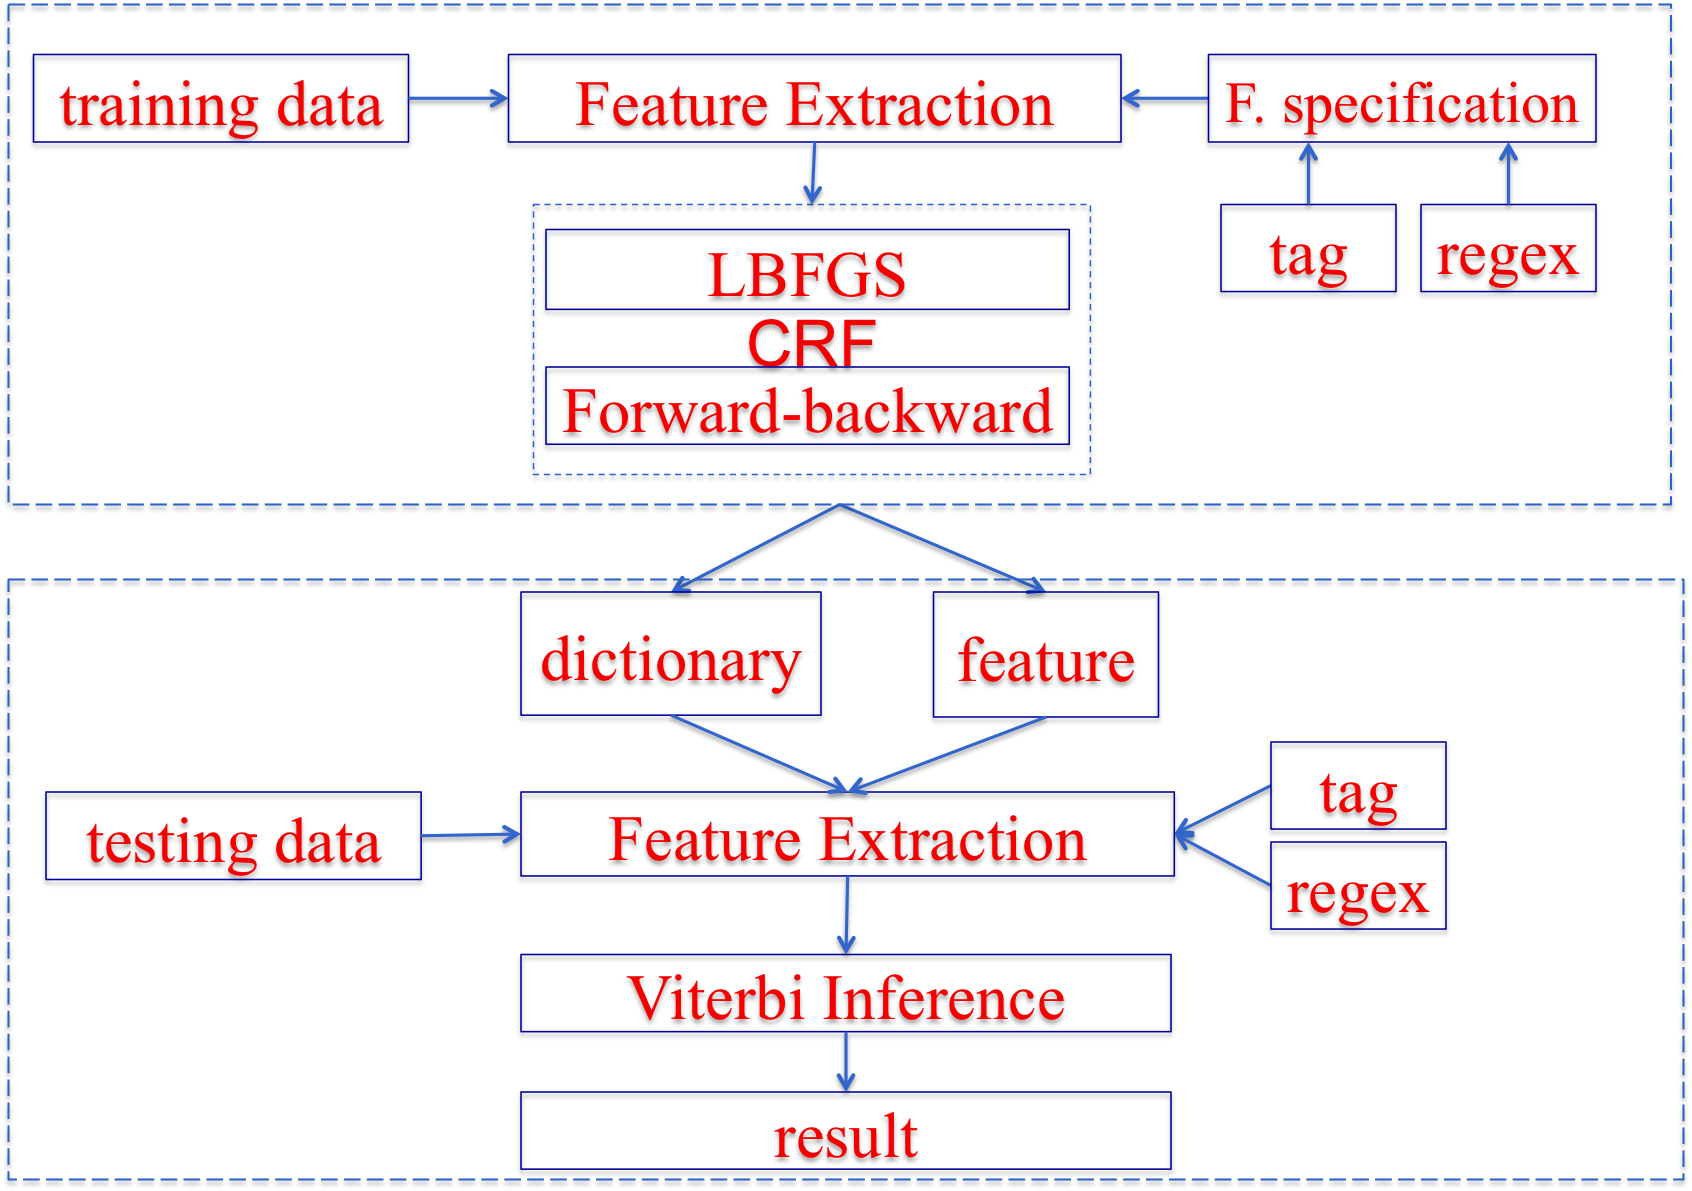
\includegraphics[height=12em]{images/system.png}
			
			}

                %%%%%%%%%%%%%%%%%%%%%%%%%%%%%%%%%%%%%%%%%%%%%%%%%%%%%%%%%%%%%%%%%%%%%%%%%%%%%%
                  \headerbox{Performance Evaluation}{name=myexperiment,column=0,below=myintroduction}{
                %%%%%%%%%%%%%%%%%%%%%%%%%%%%%%%%%%%%%%%%%%%%%%%%%%%%%%%%%%%%%%%%%%%%%%%%%%%%%%
                  %       \includegraphics[width=0.85\linewidth]{T-labs-Drawing-1} 
                          \newcommand{\compactlist}{\setlength{\itemsep}{0pt} \setlength{\parskip}{0pt} \setlength{\leftskip}{-1em}}
                          
                                        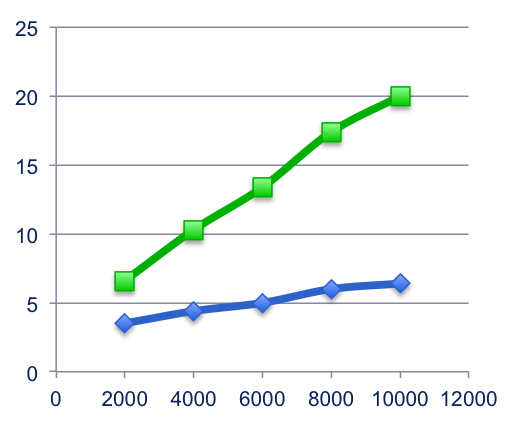
\includegraphics[height=8.5em,width=10em]{images/extraction.png}
                                        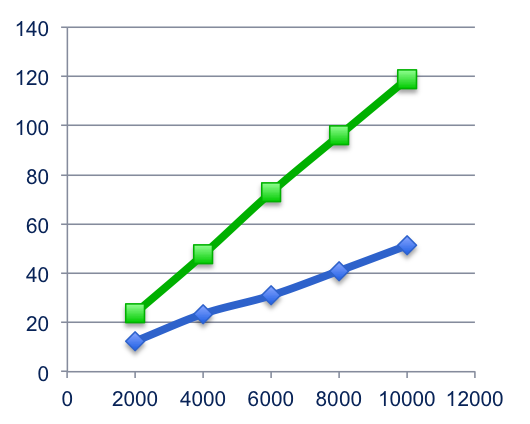
\includegraphics[height=8.5em,width=10em]{images/viterbi.png}

                }

		 %%%%%%%%%%%%%%%%%%%%%%%%%%%%%%%%%%%%%%%%%%%%%%%%%%%%%%%%%%%%%%%%%%%%%%%%%%%%%%
		  \headerbox{Acknowledgements}{name=myacknowledgements,column=0,below=myexperiment}{
		%%%%%%%%%%%%%%%%%%%%%%%%%%%%%%%%%%%%%%%%%%%%%%%%%%%%%%%%%%%%%%%%%%%%%%%%%%%%%%
		  %	  \includegraphics[width=0.85\linewidth]{T-labs-Drawing-1} 
			  \newcommand{\compactlist}{\setlength{\itemsep}{0pt} \setlength{\parskip}{0pt} \setlength{\leftskip}{-1em}}

This work is supported by EMC/Greenplum. Thanks to EMC/Greenplum employee Caleb Welton and Hitoshi Harada s 
precious feedback and code review.
	

	  	}

		%%%%%%%%%%%%%%%%%%%%%%%%%%%%%%%%%%%%%%%%%%%%%%%%%%%%%%%%%%%%%%%%%%%%%%%%%%%%%%
		  \headerbox{Parallel Text Feature Extraction}{name=myourapproach,column=1,span=3,row=0}{
		%%%%%%%%%%%%%%%%%%%%%%%%%%%%%%%%%%%%%%%%%%%%%%%%%%%%%%%%%%%%%%%%%%%%%%%%%%%%%%
			
			  \newcommand{\compactlist}{\setlength{\itemsep}{0pt} \setlength{\parskip}{0pt} \setlength{\leftskip}{-1em}}
Text feature extraction is a step in most statistical text analysis methods, and it can be an expensive operation. 
To achieve high quality, CRF methods often assign hundreds of features to each token in the document. 
Examples of such features include: (1) dictionary features: does this token exist in a provided dictionary? 
(2) regex features: does this token match a provided regular expression? 
(3) edge features: is the label of a token correlated with the label of a previous token? 
(4) word features: does this the token appear in the training data? and 
(5) position features: is this token the first or last in the token sequence? 
The right combination of features depends on the application, and so our support for feature extraction heavily 
leverages the microprogramming interface provided by MADlib.
		
			}
		%%%%%%%%%%%%%%%%%%%%%%%%%%%%%%%%%%%%%%%%%%%%%%%%%%%%%%%%%%%%%%%%%%%%%%%%%%%%%%
		  \headerbox{Parallel Linear-chain CRF Training}{name=myapproxstrmatch,column=1,span=3,below=myourapproach}{
		%%%%%%%%%%%%%%%%%%%%%%%%%%%%%%%%%%%%%%%%%%%%%%%%%%%%%%%%%%%%%%%%%%%%%%%%%%%%%%
			  \newcommand{\compactlist}{\setlength{\itemsep}{0pt} \setlength{\parskip}{0pt} \setlength{\leftskip}{-1em}}
CRF training is time consuming due to the expensive forward-backward computation to evaluate the log-likelihood
function and its gradient vector for each interation.\\
$\ell_\lambda^\prime=\sum_k[\lambda F(y_k,x_k)-\log Z_\lambda(x_k)]-\frac{\lambda^2}{2\sigma ^2}+const$\\
with gradient\\
$\nabla \ell_\lambda^\prime=\sum_k[\lambda F(y_k,x_k)-E_{p\lambda(Y|x_k)}F(Y,x_k)]-\frac{\lambda}{\sigma ^2}$\\
parallel forward-backward computation\\			
		 
		 }
		%%%%%%%%%%%%%%%%%%%%%%%%%%%%%%%%%%%%%%%%%%%%%%%%%%%%%%%%%%%%%%%%%%%%%%%%%%%%%%%
				%%%%%%%%%%%%%%%%%%%%%%%%%%%%%%%%%%%%%%%%%%%%%%%%%%%%%%%%%%%%%%%%%%%%%%%%%%%%%%%
		\headerbox{Parallel Viterbi Inference}{name=mycer,column=1,span=3,below=myapproxstrmatch}{
		%%%%%%%%%%%%%%%%%%%%%%%%%%%%%%%%%%%%%%%%%%%%%%%%%%%%%%%%%%%%%%%%%%%%%%%%%%%%%%%
The Viterbi dynamic programming algorithm [14] is the popular algorithm to find the top-k most likely labelings of a document 
for (linear chain) CRF models. Like any dynamic programming algorithm, the Viterbi algorithm is recursive. We experimented 
with two direct implementations of macro-coordination over time. First, we chose to implement it using a combination of 
recursive SQL and window aggregate functions. We discussed this implementation at some length in earlier work [42]. 
Our initial recursive SQL implementation only runs over PostgreSQL versions 8.4 and later; it does not run in Greenplum. 
Second, we chose to implement a Python UDF that uses iterations to drive the recursion in Viterbi. This iterative 
implementation runs over both PostgreSQL and Greenplum. In Greenplum, Viterbi can be run in parallel over different subsets 
of the document on a multi-core machine.We want to find the sequence of tags that maximizes the formula.\\
$P(T_1,T_2,...,T_n|W_1,W_2,...,W_n)$ which can be estimated as $\prod_{1\leq i\leq n} (P(T_i|T_{i-1})*P(W_i|T_i))$\\
$P(T_i|T_{i-1}$ is the transition weight\\
$P(W_i|T_i)$ is the emissing weight\\
-Create tables and import model data to the database
$SELECT madlib.load\_crf\_model('/path/to/modeldata')$\\
--Feature extraction
$SELECT madlib.text\_feature\_extraction$\\
--Viterbi inference\\
$SELECT madlib.vcrf\_label(...)$
Sample queries\\
$Q_1:Tagging for setence with id=501$\\
$SELECT doc\_id, madlib.vcrf\_top1\_label(mfactors.score,rfactors.score)$\\
$FROM m\_factors mfactors, r_factors rfactor;$\\
$Q_2:Tagging for all sentences containing the word 'professor'$\\
$SELECT DISTINCT ON doc\_id, madlib.vcrf\_top1\_label(mfactors.score,rfactors.score)$\\
$FROM mfactor, rfactori, seg\_tbl, segmenttbl$\\
$WHERE segtbl.doc\_id=segmenttbl.doc\_id AND segmenttbl.seg\_text='professor'$\\

		}
                %%%%%%%%%%%%%%%%%%%%%%%%%%%%%%%%%%%%%%%%%%%%%%%%%%%%%%%%%%%%%%%%%%%%%%%%%%%%%%
                  \headerbox{Reference}{name=myreference,column=1,span=3,below=mycer}{
                %%%%%%%%%%%%%%%%%%%%%%%%%%%%%%%%%%%%%%%%%%%%%%%%%%%%%%%%%%%%%%%%%%%%%%%%%%%%%%
                          \newcommand{\compactlist}{\setlength{\itemsep}{0pt} \setlength{\parskip}{0pt} \setlength{\leftskip}{-1em}}
[1] http://crf.sourceforge.net/\\
http://www.cs.berkeley.edu/~daisyw/ViterbiCRF.html\\
Xuan-Hieu Phan, Le-Minh Nguyen, and Cam-Tu Nguyen. FlexCRFs: Flexible Conditional Random Fields, 2004.
                 }
	
		\end{poster}
		
		\end{document}
